
%% bare_jrnl_compsoc.tex
%% V1.4a
%% 2014/09/17
%% by Michael Shell
%% See:
%% http://www.michaelshell.org/
%% for current contact information.
%%
%% This is a skeleton file demonstrating the use of IEEEtran.cls
%% (requires IEEEtran.cls version 1.8a or later) with an IEEE
%% Computer Society journal paper.
%%
%% Support sites:
%% http://www.michaelshell.org/tex/ieeetran/
%% http://www.ctan.org/tex-archive/macros/latex/contrib/IEEEtran/
%% and
%% http://www.ieee.org/

%%*************************************************************************
%% Legal Notice:
%% This code is offered as-is without any warranty either expressed or
%% implied; without even the implied warranty of MERCHANTABILITY or
%% FITNESS FOR A PARTICULAR PURPOSE! 
%% User assumes all risk.
%% In no event shall IEEE or any contributor to this code be liable for
%% any damages or losses, including, but not limited to, incidental,
%% consequential, or any other damages, resulting from the use or misuse
%% of any information contained here.
%%
%% All comments are the opinions of their respective authors and are not
%% necessarily endorsed by the IEEE.
%%
%% This work is distributed under the LaTeX Project Public License (LPPL)
%% ( http://www.latex-project.org/ ) version 1.3, and may be freely used,
%% distributed and modified. A copy of the LPPL, version 1.3, is included
%% in the base LaTeX documentation of all distributions of LaTeX released
%% 2003/12/01 or later.
%% Retain all contribution notices and credits.
%% ** Modified files should be clearly indicated as such, including  **
%% ** renaming them and changing author support contact information. **
%%
%% File list of work: IEEEtran.cls, IEEEtran_HOWTO.pdf, bare_adv.tex,
%%                    bare_conf.tex, bare_jrnl.tex, bare_conf_compsoc.tex,
%%                    bare_jrnl_compsoc.tex, bare_jrnl_transmag.tex
%%*************************************************************************


% *** Authors should verify (and, if needed, correct) their LaTeX system  ***
% *** with the testflow diagnostic prior to trusting their LaTeX platform ***
% *** with production work. IEEE's font choices and paper sizes can       ***
% *** trigger bugs that do not appear when using other class files.       ***                          ***
% The testflow support page is at:
% http://www.michaelshell.org/tex/testflow/


\documentclass[10pt,conference,onecolumn,compsoc]{IEEEtran}


\usepackage{hyperref}
\usepackage{enumitem}
\setlist[itemize]{leftmargin=3 cm}
\setlist[enumerate]{leftmargin=3cm}



% *** CITATION PACKAGES ***
%
\ifCLASSOPTIONcompsoc
  % IEEE Computer Society needs nocompress option
  % requires cite.sty v4.0 or later (November 2003)
  \usepackage[nocompress]{cite}
\else
  % normal IEEE
  \usepackage{cite}
\fi
% cite.sty was written by Donald Arseneau
% V1.6 and later of IEEEtran pre-defines the format of the cite.sty package
% \cite{} output to follow that of IEEE. Loading the cite package will
% result in citation numbers being automatically sorted and properly
% "compressed/ranged". e.g., [1], [9], [2], [7], [5], [6] without using
% cite.sty will become [1], [2], [5]--[7], [9] using cite.sty. cite.sty's
% \cite will automatically add leading space, if needed. Use cite.sty's
% noadjust option (cite.sty V3.8 and later) if you want to turn this off
% such as if a citation ever needs to be enclosed in parenthesis.
% cite.sty is already installed on most LaTeX systems. Be sure and use
% version 5.0 (2009-03-20) and later if using hyperref.sty.
% The latest version can be obtained at:
% http://www.ctan.org/tex-archive/macros/latex/contrib/cite/
% The documentation is contained in the cite.sty file itself.



% *** GRAPHICS RELATED PACKAGES ***
%
\ifCLASSINFOpdf
   \usepackage[pdftex]{graphicx}
 
\else
 
\fi
% graphicx was written by David Carlisle and Sebastian Rahtz. It is
% required if you want graphics, photos, etc. graphicx.sty is already
% installed on most LaTeX systems. The latest version and documentation
% can be obtained at: 
% http://www.ctan.org/tex-archive/macros/latex/required/graphics/
% Another good source of documentation is "Using Imported Graphics in
% LaTeX2e" by Keith Reckdahl which can be found at:
% http://www.ctan.org/tex-archive/info/epslatex/
%
% latex, and pdflatex in dvi mode, support graphics in encapsulated
% postscript (.eps) format. pdflatex in pdf mode supports graphics
% in .pdf, .jpeg, .png and .mps (metapost) formats. Users should ensure
% that all non-photo figures use a vector format (.eps, .pdf, .mps) and
% not a bitmapped formats (.jpeg, .png). IEEE frowns on bitmapped formats
% which can result in "jaggedy"/blurry rendering of lines and letters as
% well as large increases in file sizes.
%
% You can find documentation about the pdfTeX application at:
% http://www.tug.org/applications/pdftex









% *** PDF, URL AND HYPERLINK PACKAGES ***
%
\usepackage{url}
% url.sty was written by Donald Arseneau. It provides better support for
% handling and breaking URLs. url.sty is already installed on most LaTeX
% systems. The latest version and documentation can be obtained at:
% http://www.ctan.org/tex-archive/macros/latex/contrib/url/
% Basically, \url{my_url_here}.




\begin{document}

\title{3ly-Zium (Elysium)\\ for UTM CSCI 352}
%
%

% received ..."  text while in non-compsoc journals this is reversed. Sigh.

\author{Colin Weatherly, Blade Johnson% <-this % stops a space
}

\IEEEtitleabstractindextext{%
\begin{abstract}
This project is a video game in the 2D platformer genre. The player will run through a level, and upon each successful completion, the level is changed to increase the difficulty. The player will play through the stages in an attempt to reach high difficulty stages. The intended target is people that play video games, primarily those that stream games, as live reactions mesh well with high difficulties.
\end{abstract}

}


% make the title area
\maketitle



\IEEEdisplaynontitleabstractindextext

\IEEEpeerreviewmaketitle



\section{Introduction}



This project is a video game in the genre of 2D platformer. The goal of the game is to reach the exit of the level that the player character is placed in. The level’s layout will progressively get more complex with each clear, along with adding new hazards that increase the difficulty further. The penalty for failing a level is to be sent back to the beginning of said level, allowing the player to practice the level with every attempt.

The targeted audience for this project is people in the 18-34 age group who play video games on a regular basis. Specifically, those in the age group that livestream games. Due to the increasingly difficult challenge that the game provides, having live reactions of attempts to beat the game will provide content for the targeted audience.



\subsection{Background}
A 2D platformer is a game genre set on a 2D plane where the player controlled character must move and jump to avoid obstacles and reach the end.

We decided to make a platforming game because of our love for games in general and our shared interest in platformers. Because of this, we feel we can properly create one.

% needed in second column of first page if using \IEEEpubid
%\IEEEpubidadjcol


\subsection{Impacts}
This project is not meant to impact the world in some way. The point of a game is to provide entertainment, which will only impact a portion of the population if it were to gain traction within the community. At the current time, there is no plan for a meaningful story in the game, so the impact will be purely driven by the quality of the gameplay.

\subsection{Challenges}
The main challenges were coding the physics of the player character, developing new mechanics instead of only having the ability to move left and right and jump, and keeping the game fun despite the difficulty. Making content for streamers and making the levels increasingly challenging were also challenges.


\section{Scope}
This platforming game is considered done once three levels of the game are playable from start to finish with minimal bugs or exploits. The player should be able to get through these stages without too much unnecessary frustration with either the difficulty of these stages or the control of the player character. The player character should be fully implemented with all moves intact (moving, jumping) and all hazards(such as spikes) should fail the level upon contact with the player character. As a stretch goal, we want to include more levels with new hazards. An additional stretch goal is the addition of extra moves(i.e walljumping, sliding) the player character requires to progress in more difficult levels. An additional stretch goal is scaling the window and the game assets to fit more than one resolution.

\subsection{Requirements}
The requirements were gathered by considering the needs of the user when playing though and practicing the levels in the game. We determined what would fit best for playability and user convenience, especially in the case of a 2D platforming game. We then used these to put together specific necessities of the program.

\subsubsection{Functional}
\begin{itemize}
\item User inputs via designated keys are read – the application should register the inputs and move the player character accordingly
\item Selecting Start places the user in the first level – Unlike the level select which allows the user to choose a level, pressing the start button will immediately bring them to the first level
\item Level fails upon contact with a hazard – should the player character run into a hazard(i.e pits), level is failed and character is returned to the starting point of the same level
\end{itemize}

\subsubsection{Non-Functional}
\begin{itemize}
\item The game correctly displays in a 1280x720 resolution window
\item The game runs at a smooth framerate, preferably 30 frames per second
\item User's inputs have little to no delay, preferably under half a second
\end{itemize}

\subsection{Use Cases}
These are cases in which the user will interact with the program's user interface. The use cases can be seen in Table \ref{tab:useCaseIndex}.




\begin{table}
\centering
\begin{tabular}{|c|c|c|c|c|}
\hline
Use Case ID & Use Case Name & Primary Actor & Complexity & Priority \\
\hline \hline
1 & Start New Game & User & Low & 2\\
\hline
2 & Level Select & User & Low & 3\\
\hline
3 & Character Jump & User & Medium & 1\\
\hline
4 & Character Dash & User & Medium & 1\\
\hline

\end{tabular}
\caption{Use case table}
\label{tab:useCaseIndex}
\end{table}


\begin{itemize}
\item[Use Case Number:] 1
\item[Use Case Name:] Start New Game
\item[Description:] The player decides to begin the game from the beginning (Level 1). They will click on the ``Start" button (see Figure \ref{Start Mockup}). This will load the first level of the game (see Figure \ref{Level1 Mockup}).
\end{itemize}

Process flow:

\begin{enumerate}
\item Player starts the program, which begins with the main menu loaded.
\item The player left-clicks the ``Start" option on the menu.
\item The game state is updated to gameplay, and the first level is loaded.
\item[Termination Outcome:] Gameplay has begun in level 1.
\end{enumerate}

\begin{itemize}
\item[Use Case Number:] 2
\item[Use Case Name:] Level Select
\item[Description:] The player should be taken to a level select when selecting the option on the main menu, where they can select any level to play (see Figure \ref{Select Mockup}).
\end{itemize}

Process flow:

\begin{enumerate}
\item Player starts the program, which begins with the main menu loaded.
\item The player left-clicks the ``Level Select" option on the main menu.
\item The level select screen is loaded, showing each level vertically in numerically descending order.
\item The player left-clicks the option corresponding to their desired level.
\item The game state is updated to gameplay, and the corresponding level loads.
\item[Termination Outcome:] Gameplay has begun in the player's selected level.
\end{enumerate}

\begin{itemize}
\item[Use Case Number:] 3
\item[Use Case Name:] Character Jump
\item[Description:] The player character should jump into the air upon the player pressing the `Z' key.
\end{itemize}

Process flow:

\begin{enumerate}
\item Player is in a stage of gameplay.
\item The player presses the `Z' key.
\item The player character then leaps off the ground into the air.
\item After a few seconds of gradually rising upward, the player character then gradually falls until hitting the ground.
\item[Termination Outcome:] The player character has completed a full jump.
\end{enumerate}

\begin{itemize}
\item[Use Case Number:] 4
\item[Use Case Name:] Character Dash
\item[Description:] The character should dash forward in the direction being faced when pressing the `X` key.
\end{itemize}

Process flow:

\begin{enumerate}
\item Player is in a stage of gameplay.
\item The player presses the 'X' key.
\item The player's movement speed is doubled in the direction of movement(left, right) for a second.
\item[Termination Outcome:] The player has completed a full dash.
\end{enumerate}


\subsection{Interface Mockups}
In Figure \ref{Level1 Mockup}, this shows the player character (in the top left corner of the mockup) standing in the initial state when Level 1 begins. The character can traverse the platforms (the graphical rectangles that stick out from the background) to reach the right of the screen (which is where the goal would be). Falling in the pit would send you back to that position.
Figure \ref{Start Mockup} shows the title screen that you see upon starting the program. The three options under the graphic (from left to right) start you into Level 1, take you to the level select screen, and close the program respectively.
Figure \ref{Select Mockup} shows the level select which you can reach from the title screen's middle option. Selecting ``Level 1," ``Level 2," or ``Level 3" will start the player in the corresponding level of the game.
\begin{figure}[ht!]
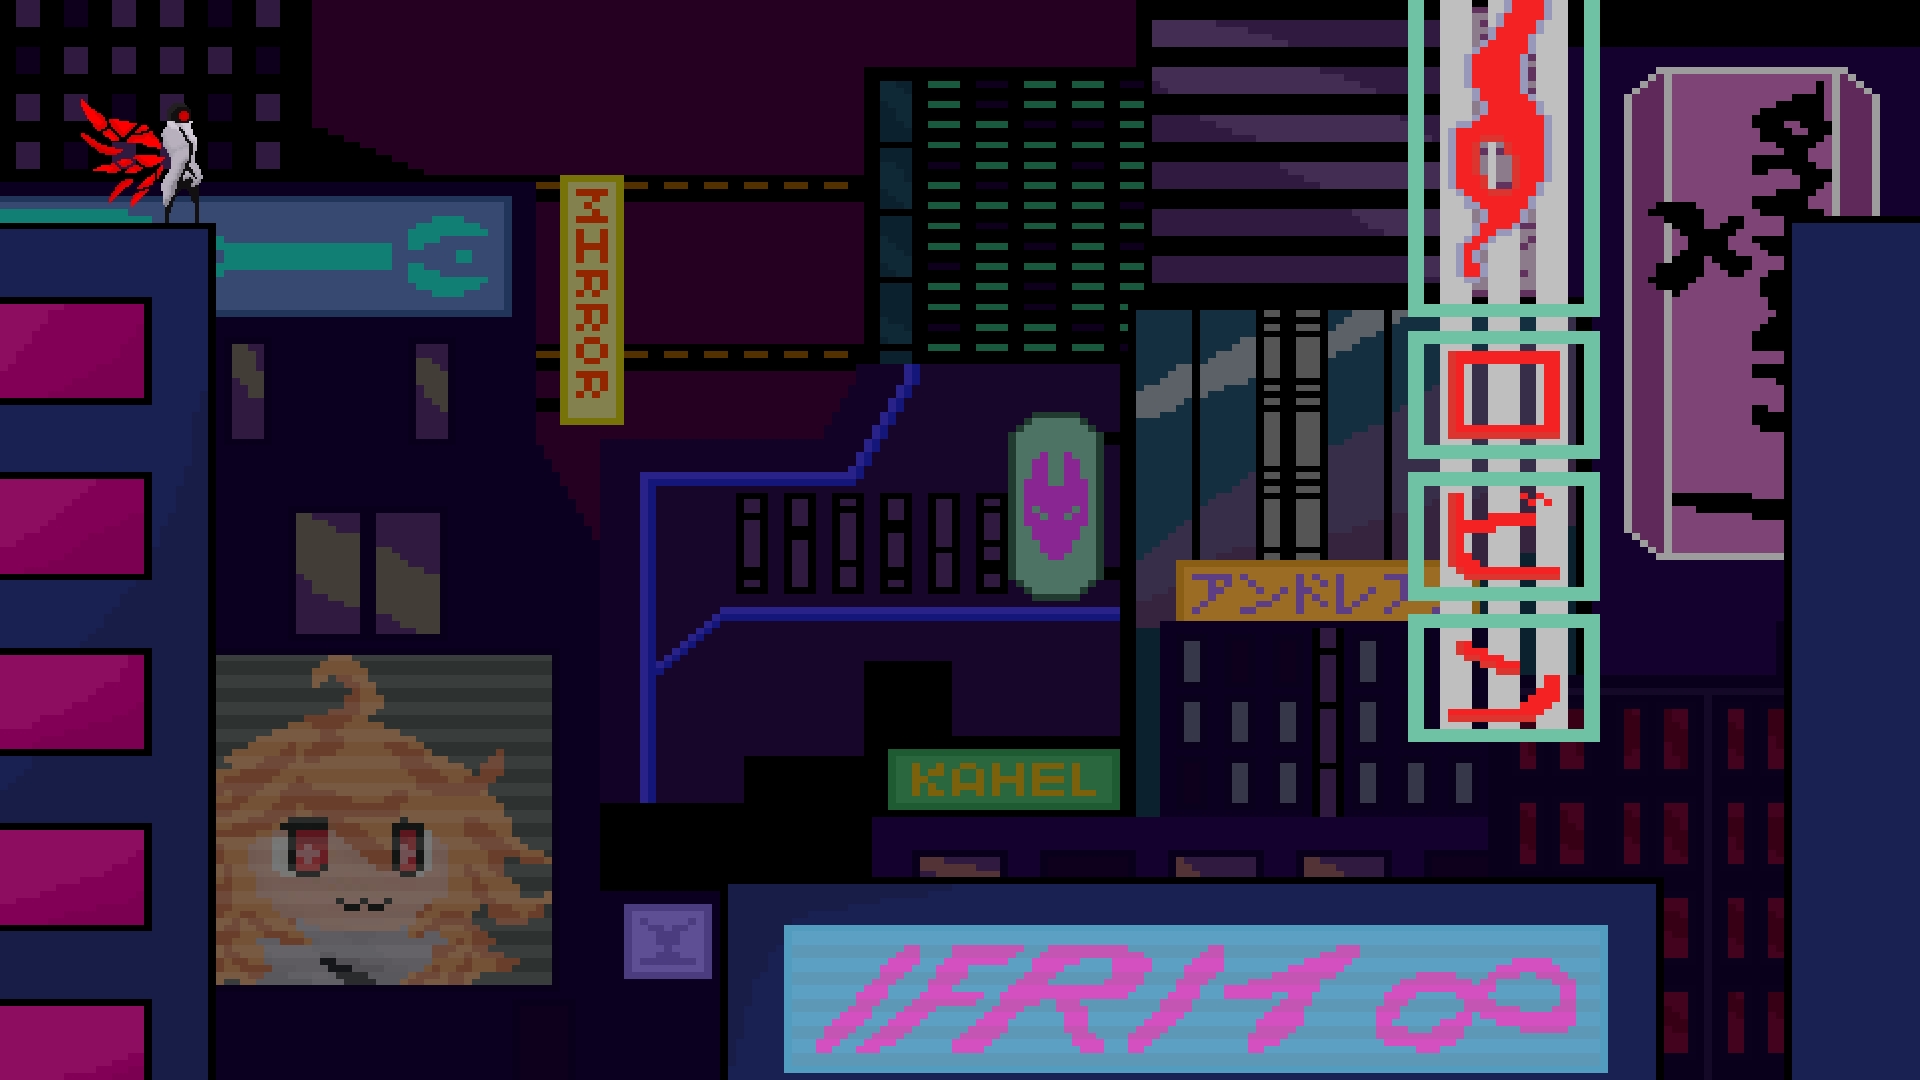
\includegraphics[height=250px, width=400px]{Level1 Mockup.png}
\caption{Mockup of a player loading into level 1}
\label{Level1 Mockup}
\end{figure}

\begin{figure}[ht!]
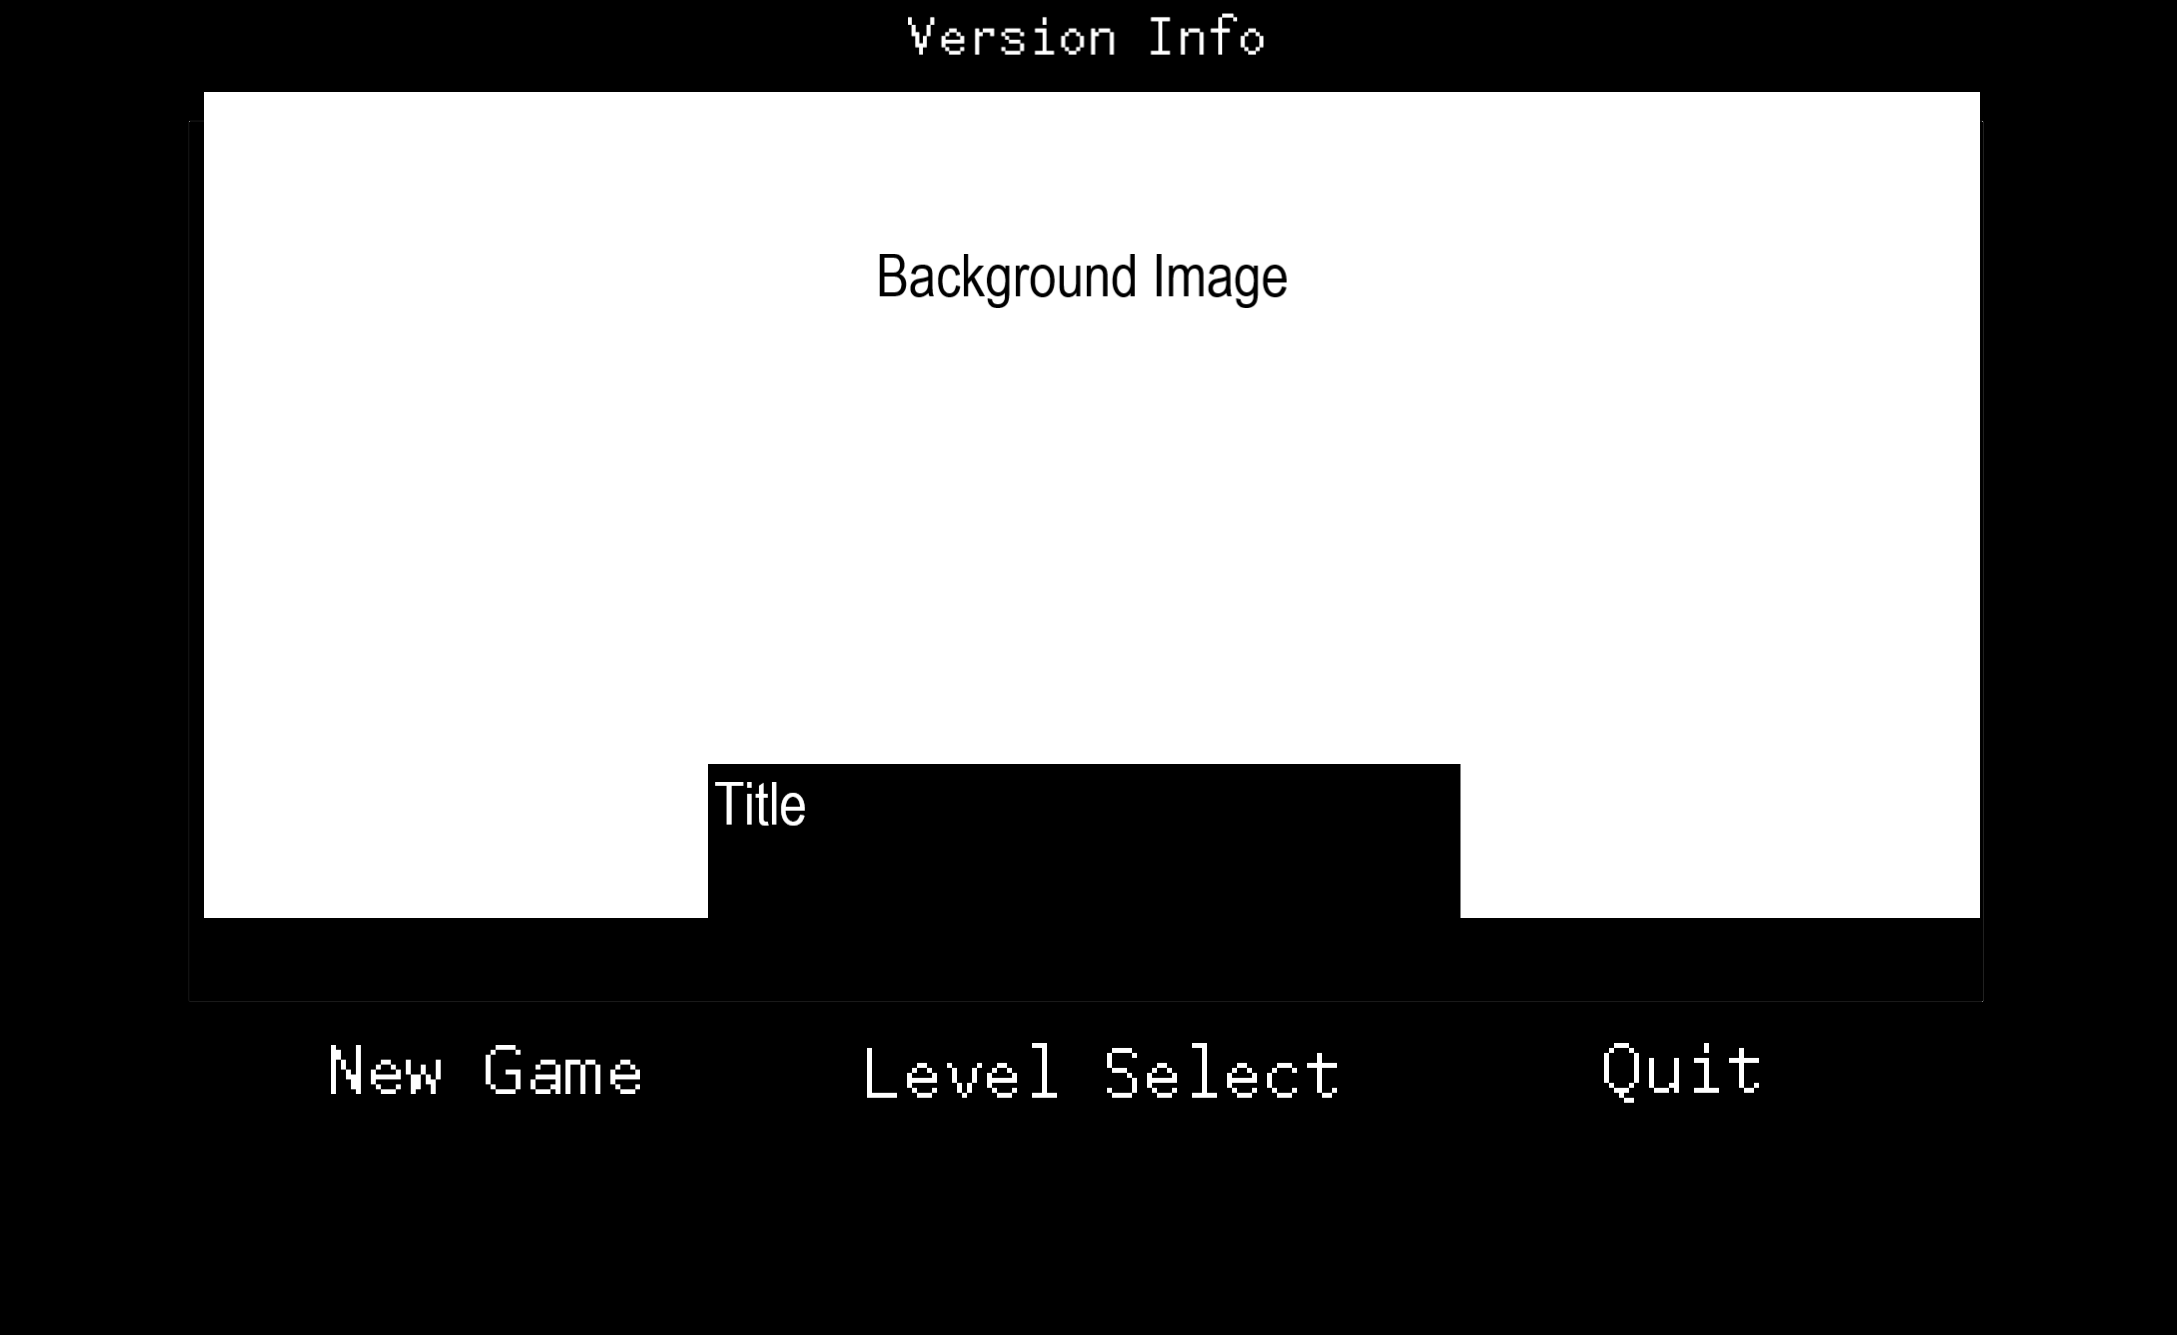
\includegraphics[height=250px, width=400px]{Start Mockup.png}
\caption{Mockup of the main menu screen}
\label{Start Mockup}
\end{figure}

\begin{figure}[ht!]
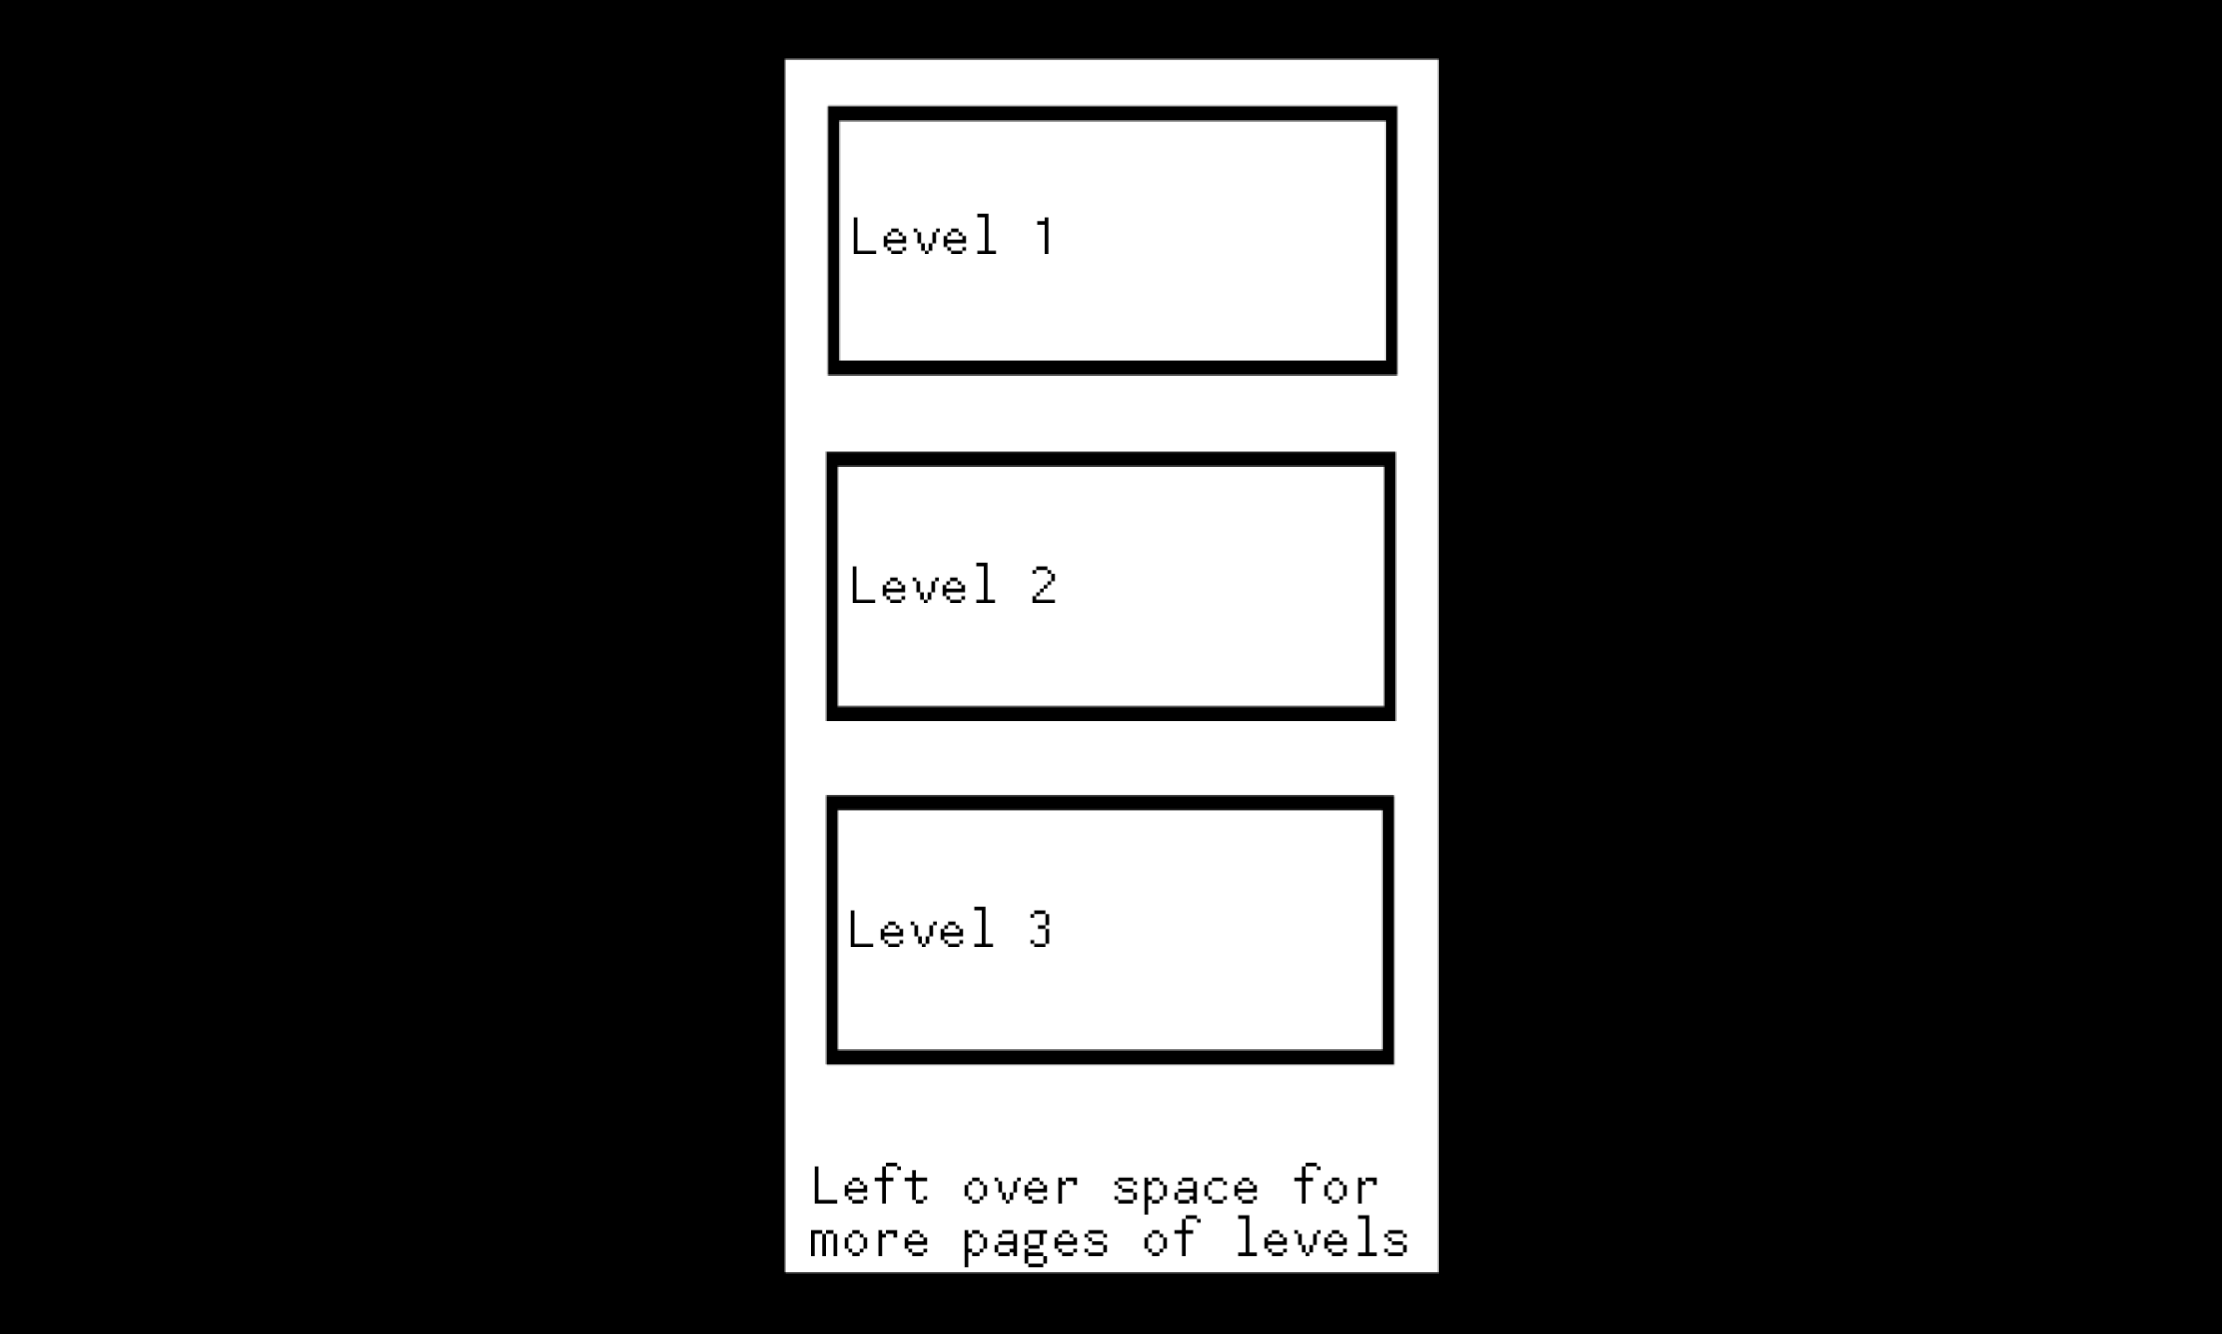
\includegraphics[height=250px, width=400px]{Select Mockup.png}
\caption{Mockup of the level select screen}
\label{Select Mockup}
\end{figure}



\section{Project Timeline}
Refer to Figure \ref{Timeline}.

February 5th is where we propose the idea of a 2D platformer game.

March 1st sees us writing up use cases and setting requirements. Concepts are put into place with mockups being created.

March 28th is when the project is updated with designs that are more fleshed out and close to final. Initial structure ideas are outlined in a preliminary UML.

April 8th has movement being more or less completed, with wall and ground collision now being worked on.

April 15th has collision being finished or nearly finished. Level loading has begun implementation or is approaching implementation.

April 22nd has level loading finished or nearing completion. Menus have begun implementation. Bug testing has begun.

Lastly, April 28th has the project being completed, having met all goals and running with few bugs.
\begin{figure}[ht!]
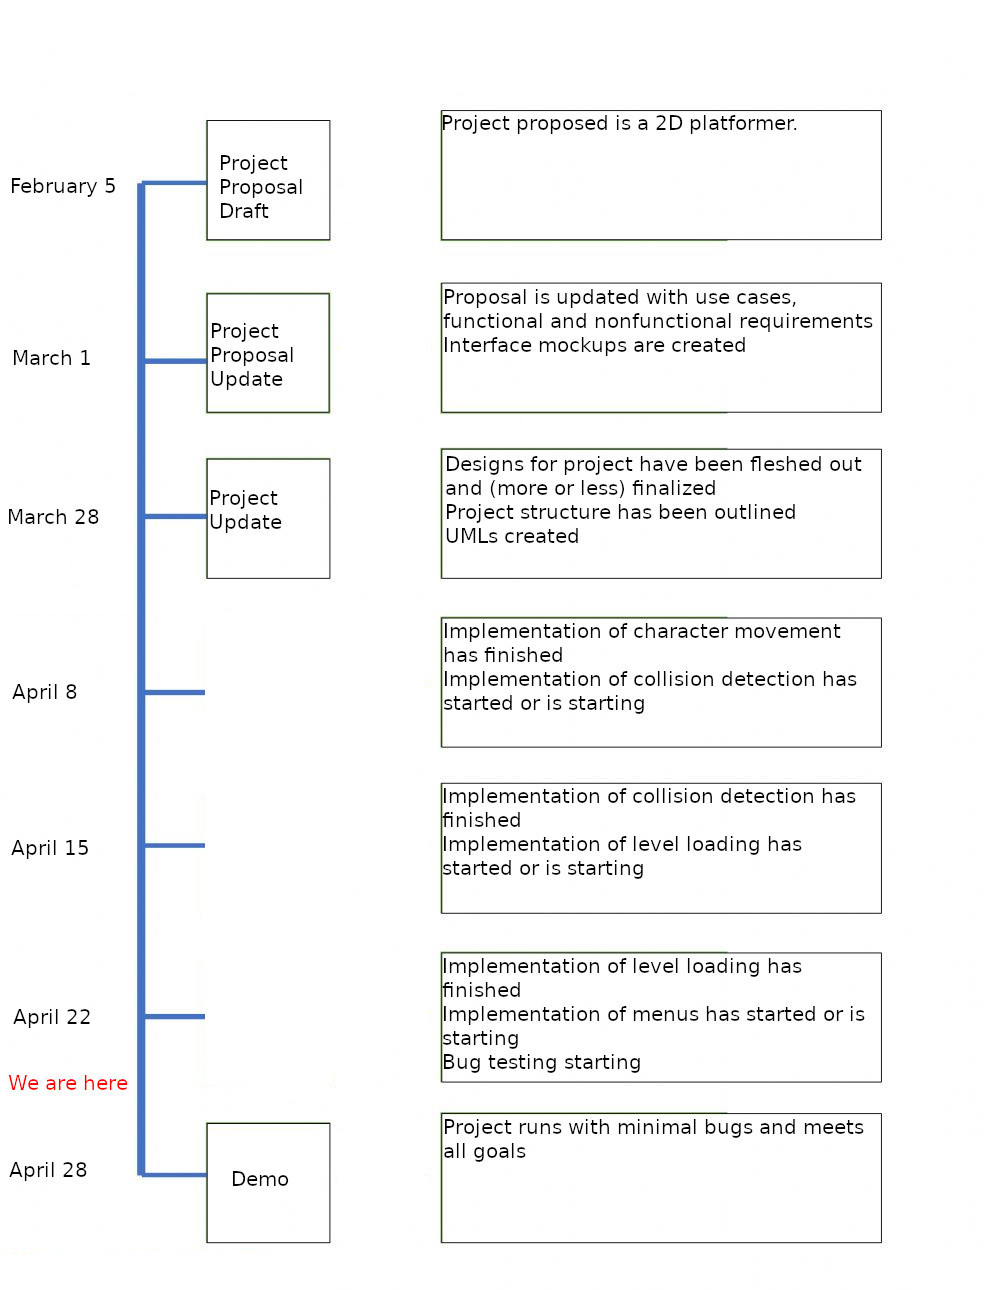
\includegraphics[height=400px, width=300px]{Timeline.jpg}
\caption{Timeline}
\label{Timeline}
\end{figure}


\section{Project Structure}
Our overall approach was to make a game that featured simple menus that can head straight into gameplay or start gameplay at any point in the game.

From main, the menus will be loaded. From here, the Window1 class (Level Select) will contain methods for all of the choices, which will start the game, access the Window2 class (Level Select), or close the program. The Window1 and Window2 classes can both load into the gameplay. Window3, Window4, and Window5 classes (Levels 1, 2, and 3) run the gameplay. These three classes contain the information for the character as well as level data and collision data. The MusicClass also plays music for the game in the background in each screen.

- MusicClass: We decided to make MusicClass a separate class so that it could be easily instantiated in any class and play the required music.

- QuitDecorator: We decided to add this as a small detail when you exit the game. We wanted to have a "Thanks for playing!" message to let the user know we appreciate the time they took to play it.

- Graphical Direction: We decided on a sci-fi style art directions with a neon city in the background and a robotic-looking main character. This mostly came about from graphical experiments, but it ended up sticking.

\subsection{UML Outline}
Refer to Figure \ref{Facade}.

Window1 (title screen) is what the user loads into upon start up, as MainOverride creates an instance of Window1. Button\_Click\_1 creates an instance of LevelSelect, which allows users to start from any level in the game, and Button\_Click\_2 loads an instance of Window3 (Level 1). Button\_Click\_3 simply closes the program.

Window is where the user can select any of the 3 levels. Button\_Click\_1 creates an instance of Window3, starting you in the first level. Button\_Click\_2 creates an instance of Window4, starting you in the second level. Lastly, Button\_Click\_3 creates an instance of Window5, starting you in the third level.

The MusicClass creates a music player in each of the windows it is instantiated in (Window1, Window3, Window4, Window5). This allows these screens/sections of the game to have music played in the background.

QuitDecorator is a class that decorates the Button used for quitting out of the program on the title screen. It allows the button to display an extra message when sent, which is "Thanks for playing!"

Each of the 3 level Windows (Window3, Window4, Window5) contain all of the data for that level as well as how the player collides with the level. Upon completing each level, the next is loaded.
\begin{figure}[ht!]
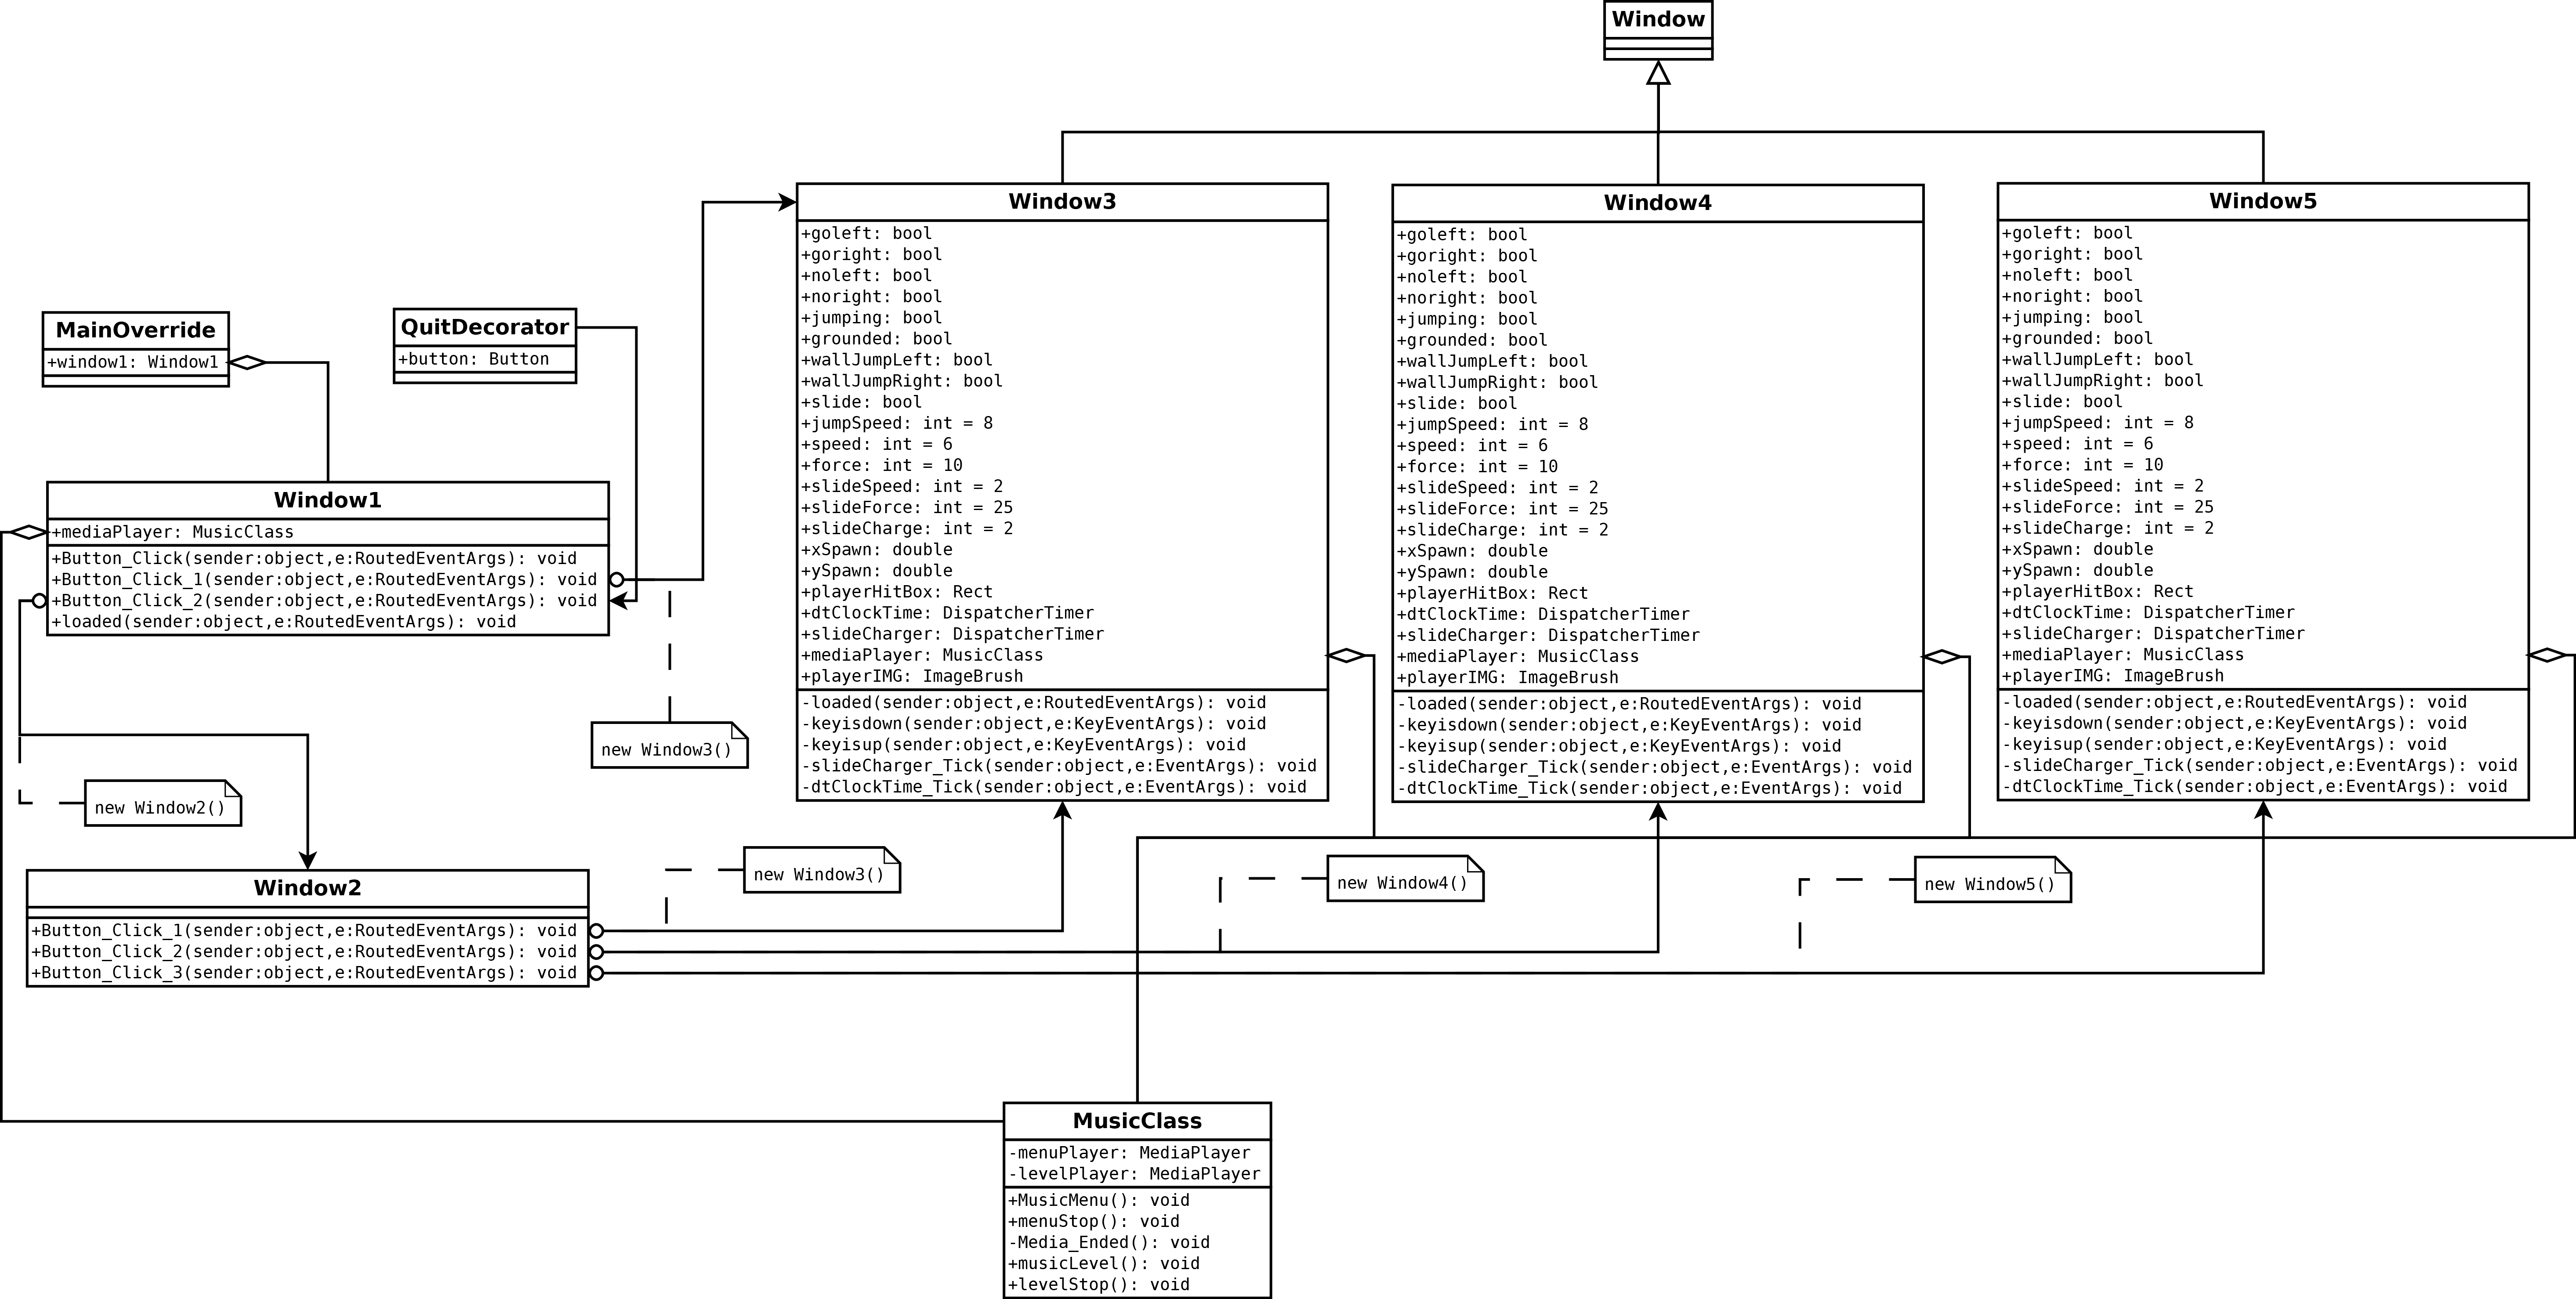
\includegraphics[height=250px, width=500px]{elyzium_uml.png}
\caption{UML Outline}
\label{Facade}
\end{figure}



\subsection{Design Patterns Used}
The 2 design patterns used are the Factory pattern and the Decorator pattern.

Factory: Your selection from Window2 (Level select window) will create an instance of one of the three levels depending on the selection.

Decorator: A QuitDecorator decorates one of the buttons on Window1 (title screen) to add extra functionality. In this case, it adds a ``Thanks for playing!" message whenever clicking it.


\section{Results}
While the project was difficult in some places to create, things came together fairly well. We were able to present the project in full on April 28th, and it seemed to have gotten some positive looks from people. In the end, we ended up satisfying all requirements we need and finished the project. The game is fully-functional and can be completed from beginning to end. While we were not able to act on many stretch goals before the presentation on April 28th, we had a good amount to show regardless. A refactor was in the works for certain parts of the project, but was not able to be completed, as work for the main branch was being updated simultaneously, and we weren't able to keep the refactor up-to-date. Due to this, some code in the main branch still remains the slightest bit messy.

\subsection{Future Work}
From here, we plan to potentially clean up what we have even further. After all is said and done with this project, we don't have any particular plans to do anything more with this project when it comes to distribution or anything else. We figure this will just remain as a past project, and will be included in our portfolios. 










% that's all folks
\end{document}


